\subsection{Thermal Expansion Analysis}

The fuel and cladding form a coupled system, with the gap between them playing a crucial role in heat transfer, mechanical interactions, and safety. Accurate evaluation of thermal expansion is essential to ensure efficient operation and structural integrity of the reactor core. The calculations consider material-specific thermal expansion coefficients and the temperature distributions derived from reactor operational data.

\subsubsection{Axial Temperature Profile of the Fuel and Axial Profile of Fuel Radius (Cold vs. Hot Geometry)}

The fuel's axial temperature profile under hot operational conditions is shown in Figure \ref{fig:Fuel_Temperature_Hot}. It illustrates the temperature distribution along the fuel height, which is essential for understanding thermal stresses and expansion. We can see that the material’s expansion follows perfectly the fuel temperature profile (Figure \ref{fig:Fuel_Radius_ColdHot}).

\begin{figure}[H]
\centering
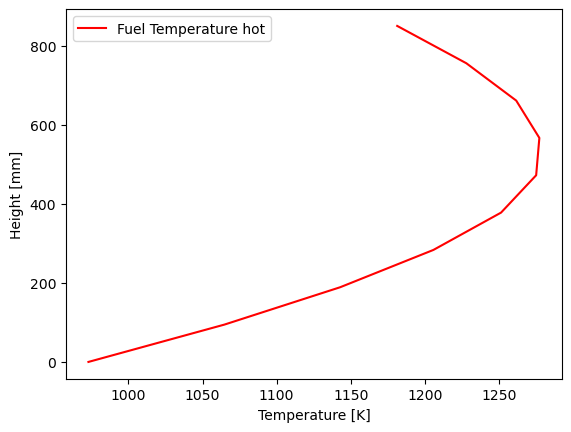
\includegraphics[width=0.8\textwidth]{1a_fuel_hot.png}
\caption{Axial temperature profile of the fuel under hot conditions.}
\label{fig:Fuel_Temperature_Hot}
\end{figure}

\begin{figure}[H]
\centering
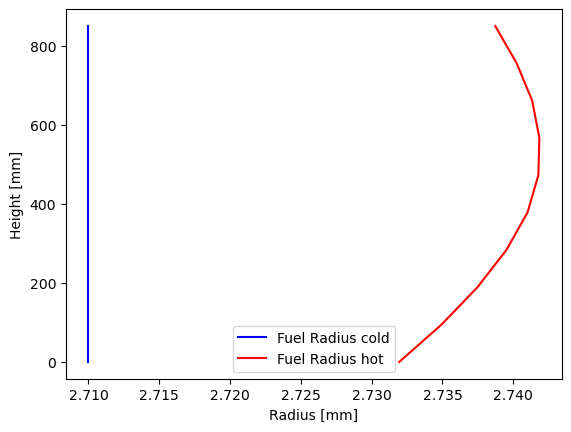
\includegraphics[width=0.8\textwidth]{1b_fuel_coldhot.png}
\caption{Axial profile of fuel radius (cold vs. hot geometry).}
\label{fig:Fuel_Radius_ColdHot}
\end{figure}

\subsubsection{Axial Temperature Profile of the Inner and Outer Cladding (Cold vs. Hot Geometry)}

The inner and outer temperature profiles of the cladding show the thermal distribution along its axial height. These graphs highlight the uniform expansion of the cladding along its height (Figure \ref{fig:Cladding_InOut_Temperature_Hot}). The temperature difference between the inner and outer part is uniform, as shown in Figure \ref{fig:Cladding_Radius_ColdHot}.

\begin{figure}[H]
\centering
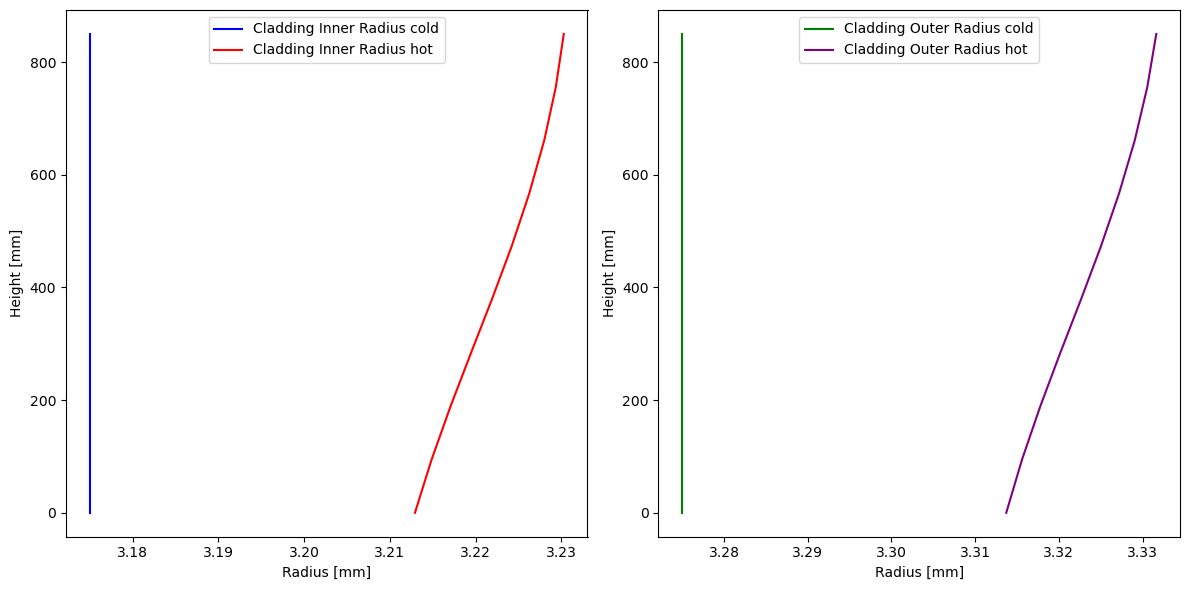
\includegraphics[width=0.8\textwidth]{2_cladding_in_out_coldhot.png}
\caption{Axial temperature profile of the cladding (cold vs. hot geometry).}
\label{fig:Cladding_InOut_Temperature_Hot}
\end{figure}

\begin{figure}[H]
\centering
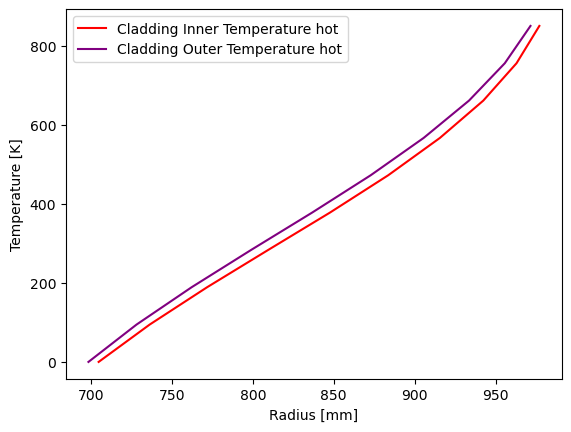
\includegraphics[width=0.8\textwidth]{3_clad_inout_diff.png}
\caption{Axial profile of cladding radius (cold vs. hot geometry).}
\label{fig:Cladding_Radius_ColdHot}
\end{figure}

\subsubsection{Gap and Cladding Thickness Along Axial Height}

The evolution of the fuel-cladding gap due to differential expansion is shown in Figure \ref{fig:Gap_Cladding_Thickness}. This parameter directly impacts heat transfer efficiency and mechanical interactions in the reactor core. The change in cladding thickness with temperature is minimal compared to the change in radius. However, it is still a key parameter for evaluating structural integrity.

\begin{figure}[H]
\centering
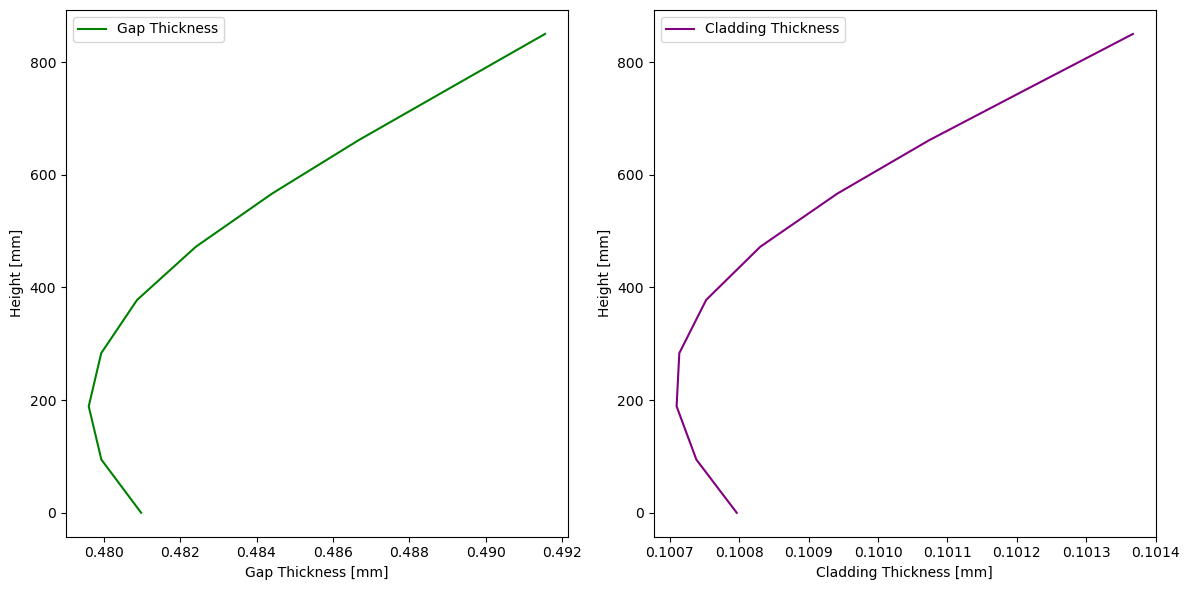
\includegraphics[width=0.8\textwidth]{4_gap_clad_thickness.png}
\caption{Gap and cladding thickness along the axial height.}
\label{fig:Gap_Cladding_Thickness}
\end{figure}

\subsubsection{Discussion}

As expected, the fuel's thermal expansion is more pronounced due to its higher temperature gradient compared to the cladding. The gap between the fuel and cladding decreases, which improves thermal coupling but must be managed carefully to avoid mechanical interactions that could compromise the system's integrity.
